\section{Grundkonzept}
\label{chap:grundkonzept}
\begin{figure}[h]
	\centering
	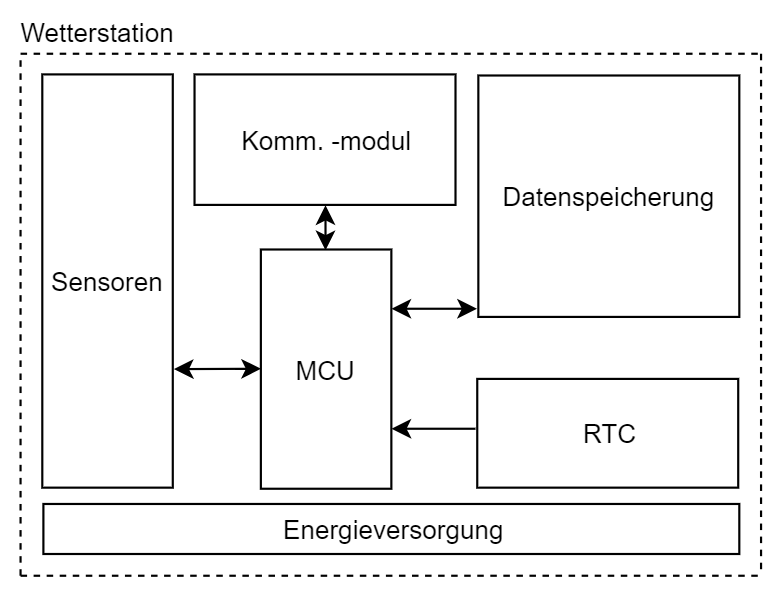
\includegraphics[width=0.9\textwidth]{graphics/Grundkonzept.PNG}
	\caption{Grundkonzept}
	\label{fig:grundkonzept}
\end{figure}

\paragraph{Übersicht:}
Als Zentralrecheneinheit wird eine \textit{Micro-Controller-Unit (MCU)} verwendet. Dieser ist dafür verantwortlich, dass die Daten richtig verarbeitet und an das dementsprechende Modul weitergeleitet werden. Die Messdaten werden in digitaler Form vom Modul \textit{Sensoren} an die \textit{MCU} übertragen. Dieser fügt mit dem \textit{Real-Time-Clock (RTC)} einen Timestamp hinzu, wobei anschließend die Daten in der \textit{Datenspeicherung} nichtflüchtig gespeichert werden. Über das \textit{Kommunikationsmodul} können dann die Daten von Nutznießern abgefragt werden.

Das gesamte Grundkonzept ist, wie in der Abbildung \ref{fig:grundkonzept} grafisch dargestellt, modular aufgebaut. Auf alle einzelnen Module wird folgend spezifischer eingegangen und die Konzeptvariationen vorgestellt. Dafür sind zusätzlich noch Vor- \& Nachteile für die Varianten aufgelistet.\\
\newpage

\subsection{Micro Controller Unit (MCU)}
\paragraph{Variante 1:}
\begin{wrapfigure}{r}{0.5\textwidth}
  \vspace{-10pt}
  \begin{center}
    \includegraphics[width=0.38\textwidth]{graphics/arduino_mega.png}
  \end{center}
  \vspace{-10pt}
  \caption{Arduino Mega \cite{Elektronik}}
  \vspace{-10pt}
  \label{fig:arduino_mega}
\end{wrapfigure}
Für die \textit{MCU} wird ein Microcontroller mit bereits vorhandener Peripherie verwendet, welcher ähnlich wie der in Abbildung \ref{fig:arduino_mega} ersichtliche Arduino Mega aufgebaut sein wird.

\paragraph{Variante 2:}
Es wird ein separates Printed Circuit Board (PCB) für die \textit{MCU} designed.\\

\begin{table}[h]
  \centering
  \label{tab:mcu}
  \small
  \caption{Vor- \& Nachteile}
    \begin{tabular}{c|l|l}
          & \textbf{Vorteile} & \textbf{Nachteile} \\
    \toprule
    \multirow{4}[2]{*}{\textbf{Variante 1}} & • In-system Programmierung & • Etwas teurer (ca. 20.- CHF) \\
          & \hspace{0.3cm} über USB Typ B möglich &  \\
          & • USB-Schnittstelle für eine &  \\
          &   \hspace{0.3cm} Datenkommunikation mit PC &  \\
          & • Erweiterbar über bereits  &  \\
          &   \hspace{0.3cm} existierende Anschlüsse &  \\
    \hline
    \multirow{3}[1]{*}{\textbf{Variante 2}} & • Keine unnötige Peripherie & • Zusätzliches Gerät (z.B. AVR Dragon) für \\
          & • Dimensionierungsänderungen & \hspace{0.3cm} eine in-system Programmierung notwendig \\
          & \hspace{0.3cm} möglich & • Zeitintensive Entwicklung\\
    \end{tabular}%
  \label{tab:mcu}%
\end{table}%

\newpage
\subsection{Sensoren}
\begin{figure}[h]
\centering
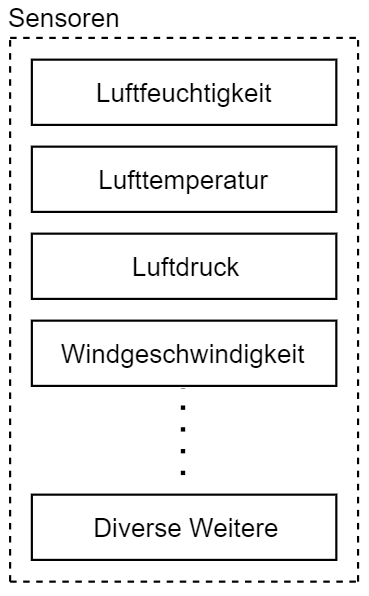
\includegraphics[scale=0.8]{graphics/Sensoren.PNG}
\caption{Sensoren}
\label{fig:sensoren}
\end{figure}
In dem Block \textit{Sensoren} werden alle Messeinheiten untergebracht. Die Idee dieses Blockes besteht darin, dass dieser adaptiv ist und somit leicht erweitert werden kann (Abbildung \ref{fig:sensoren}). Jeder Sensor ist nach dem Prinzip, wie in der Abbildung \ref{fig:sensoraufbau} gezeigt, aufgebaut. Es wird dann von der Seite des \textit{MCU}s aus mit dem Datenlogger kommuniziert.\\

\begin{figure}[h]
\centering
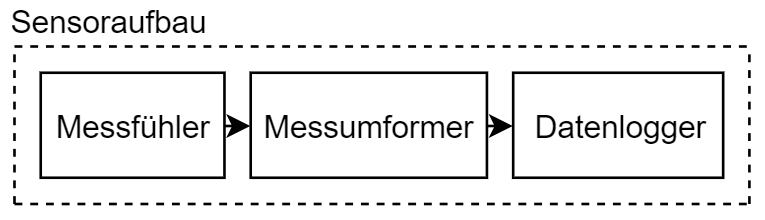
\includegraphics[scale=0.7]{graphics/Sensoraufbau.PNG}
\caption{Sensoraufbau}
\label{fig:sensoraufbau}
\end{figure}

\paragraph{Variante 1:}

Bis auf die Fühler werden die Sensoren selbst entwickelt. Dafür werden die Sensoren für die Windstärke, Lufttemperatur, Regenmenge und  Sonnenstunden gebaut.\\

\subparagraph{Windstärke:}
Die einfachste Möglichkeit ist die Windstärke über ein Schalenanenometer zu bestimmen. Mittels Reed-Kontakt oder Lichtschranke wird die Drehfrequenz bestimmt und daraus eine Windstärkenstufe nach der Beaufort-Skala zugeordnet.\\

\subparagraph{Lufttemperatur:}
Auf einem PCB wird ein IC-Bauteil zur Lufttemperaturmessung implementiert. Über einen Messumformer nach Abbildung \ref{fig:sensoraufbau} wird das Signal zur Interpretation/Auslesung für den Datenlogger aufbereitet.\\

\subparagraph{Regenmenge:}
Für die Bestimmung der Regenmenge hat sich das Kipplöffelprinzip als äußerst effizient bewiesen. Über einen Reed-Kontakt wird die Kippfrequenz bestimmt, und daraus kann auf die Regenmenge zurück geschlossen werden.\\

\subparagraph{Sonnenstunden:}
Die Sonnenstunden benötigen keinen separaten Sensor. Es ist möglich, die Länge und Intensität der Bestrahlung über die Photovoltaik zu bestimmen. Dafür muss lediglich das von der Photovoltaik zugeführte Stromsignal abgegriffen werden.\\

\paragraph{Variante 2:}

Die Sensoren werden als intelligente Wettersensorik gekauft. Diese sind, je nach Typ, in verschiedenen Variationen mit unterschiedlichen Messparametern und -technologien ausgestattet. Zudem kompatibel für den Solarbetrieb in allen Klimazonen und Wartungsfrei\footnote{abhängig von den einzelnen Sensoren}.\\

\newpage
\paragraph{Variante 3}

Eine Mischung aus den Varianten 1 \& 2.\\

\begin{table}[h]
  \centering
  \label{tab:mcu}
  \small
  \caption{Vor- \& Nachteile}
    \begin{tabular}{c|l|l}
          & \textbf{Vorteile} & \textbf{Nachteile} \\
    \toprule
    \multirow{4}[2]{*}{\textbf{Variante 1}} & • Günstig & • Sehr arbeitsaufwändig \\
          &  & • Eingeschränkt, da einzelne Messfühler \\
          &  & \hspace{0.3cm} erhältlich sind \\
          &  & • sehr Zeitaufwendig \\
    \hline
    \multirow{2}[1]{*}{\textbf{Variante 2}} & • Wartungsfreie Varianten & • Hohe Investitionskosten \\
          & • Kompatibel für Solarbetrieb & • Machbarkeitsanalyse erforderlich \\
    \hline
    \multirow{4}[1]{*}{\textbf{Variante 3}} &  &   \\
          & •  Je nach Kombination & •  Je nach Kombination  \\
          &    &  \\
    \end{tabular}%
  \label{tab:sensoren}
\end{table}
Tabelle \ref{tab:sensoren} zeigt Vor- und Nachteile für die erwähnten Varianten.\\
%\input{sections/technical/subsections/einzelne_Sensoren}

\subsection{Kommunikationsmodul}
\begin{figure}[h]
\centering
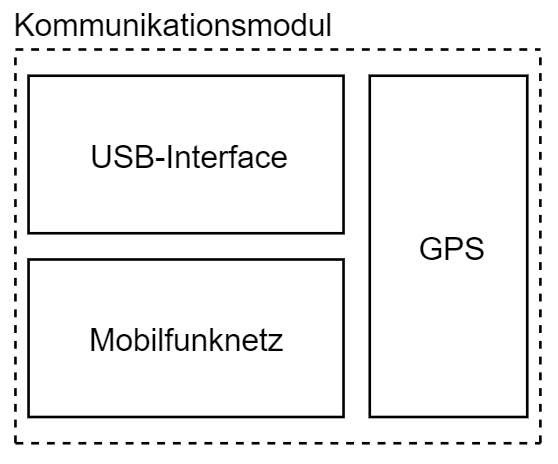
\includegraphics[scale=0.7]{graphics/Kommunikationsmodul.PNG}
\caption{Kommunikationsmodul}
\label{fig:kommunikationsmodul}
\end{figure}
Abbildung \ref{fig:kommunikationsmodul} zeigt die verschiedenen Schnittstellen, über welche Daten mit der Umgebung (User) und \textit{MCU} ausgetauscht werden können. Im Rahmen des Projekts 5 wird nur das USB-Interface umgesetzt. Mobilfunknetz und GPS sind Teil des Projekts 6.\\

\subparagraph{USB-Interface:}
Über dieses Interface kann mit dem System kommuniziert und interagiert werden.\\

\subparagraph{Mobilfunknetz:}
Die Einbindung der Wetterstation wird über diesen Block implementiert.\\

\subparagraph{GPS:}
Dieser Block sorgt für die Standortbestimmung.\\

\subsection{Datenspeicherung}
\paragraph{Variante 1:}

Die Datenspeicherung erfolgt auf einer $\mu$SD-Karte. Diese kann in ein Breakoutboard eingeschoben werden.\\

\paragraph{Variante 2:}

Es werden zur Datenspeicherung EEPROM's benutzt.\\

\begin{table}[h]
  \centering
  \label{tab:datenspeicherung}
  \small
  \caption{Vor- \& Nachteile}
    \begin{tabular}{c|l|l}
          & \textbf{Vorteile} & \textbf{Nachteile} \\
    \toprule
    \multirow{4}[2]{*}{\textbf{Variante 1}} & • Internes level-shifting & • Es wird ein zusätzliches \\
          & • Grosser Speicherplatz & \hspace{0.3cm}Breakoutboard verwendet \\
          & • Daten können notfalls auch &  \\
          &   \hspace{0.3cm} direkt von der $\mu$SD-Karte &  \\
          &   \hspace{0.3cm} entnommen werden &  \\
    \hline
    \multirow{2}[1]{*}{\textbf{Variante 2}} &       & • Kleiner Speicherplatz \\
          &       & • Benötigt level-shifting \\
    \end{tabular}%
  \label{tab:Datenspeicherung}%
\end{table}%

Tabelle \ref{tab:Datenspeicherung} zeigt Vor- und Nachteile für die erwähnten Varianten.\\

\subsection{RTC}
Es wird eine RTC implementiert, welche aktuelle Zeitstempel für erhobene Datensätze ermittelt.\\

\subsection{Energieversorgung}
\begin{figure}[h]
\centering
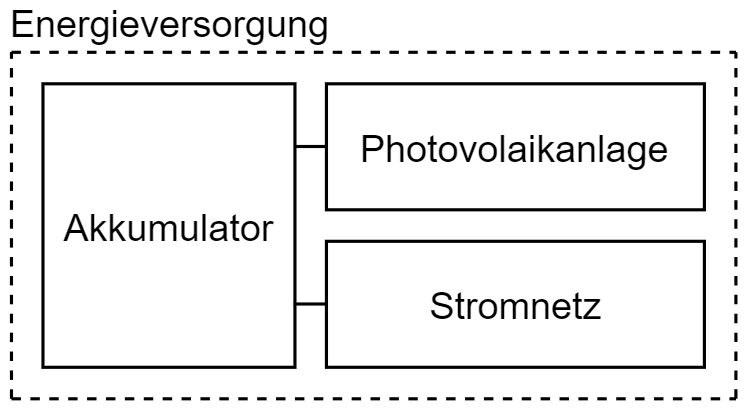
\includegraphics[scale=0.6]{graphics/Energieversorgung.PNG}
\caption{Energieversorgung}
\label{fig:Energieversorgung}
\end{figure}

Für die Speisung wird ein Akku verwendet. Gemäss Abbildung \ref{fig:Energieversorgung} soll dieser durch eine Photovoltaikanlage geladen werden. Als Wunschziel soll der Akku austauschbar ist.\\